\documentclass[10pt]{article}
\usepackage[utf8]{inputenc}
\usepackage[T1]{fontenc}
\usepackage{amsmath}
\usepackage{amsfonts}
\usepackage{amssymb}
\usepackage{mhchem}
\usepackage{stmaryrd}
\usepackage{graphicx}
\usepackage[export]{adjustbox}
\graphicspath{ {./images/} }

\begin{document}
\section{Contents}
1 Convolutional Neural Networks $\ldots \ldots \ldots \ldots \ldots \ldots \ldots$

1.1 Some classic CNN models $\ldots \ldots \ldots \ldots \ldots \ldots \ldots \ldots \ldots$

1.1.1 LeNet-5, AlexNet and VGG $\ldots \ldots \ldots \ldots . . . . . . . . . . . .$

$1.1 .2 \quad$ ResNet $\ldots . \ldots . . . . . . . . . . . . . . . . . . . . . . . . . . . . . . .$

1.1.3 pre-act ResNet $\ldots \ldots \ldots \ldots \ldots \ldots \ldots \ldots . . . . . . . . . . . . . . . . . . . . . . . . . . .$

References $\ldots \ldots \ldots \ldots \ldots \ldots \ldots \ldots \ldots \ldots \ldots \ldots \ldots \ldots \ldots \ldots \ldots \ldots$

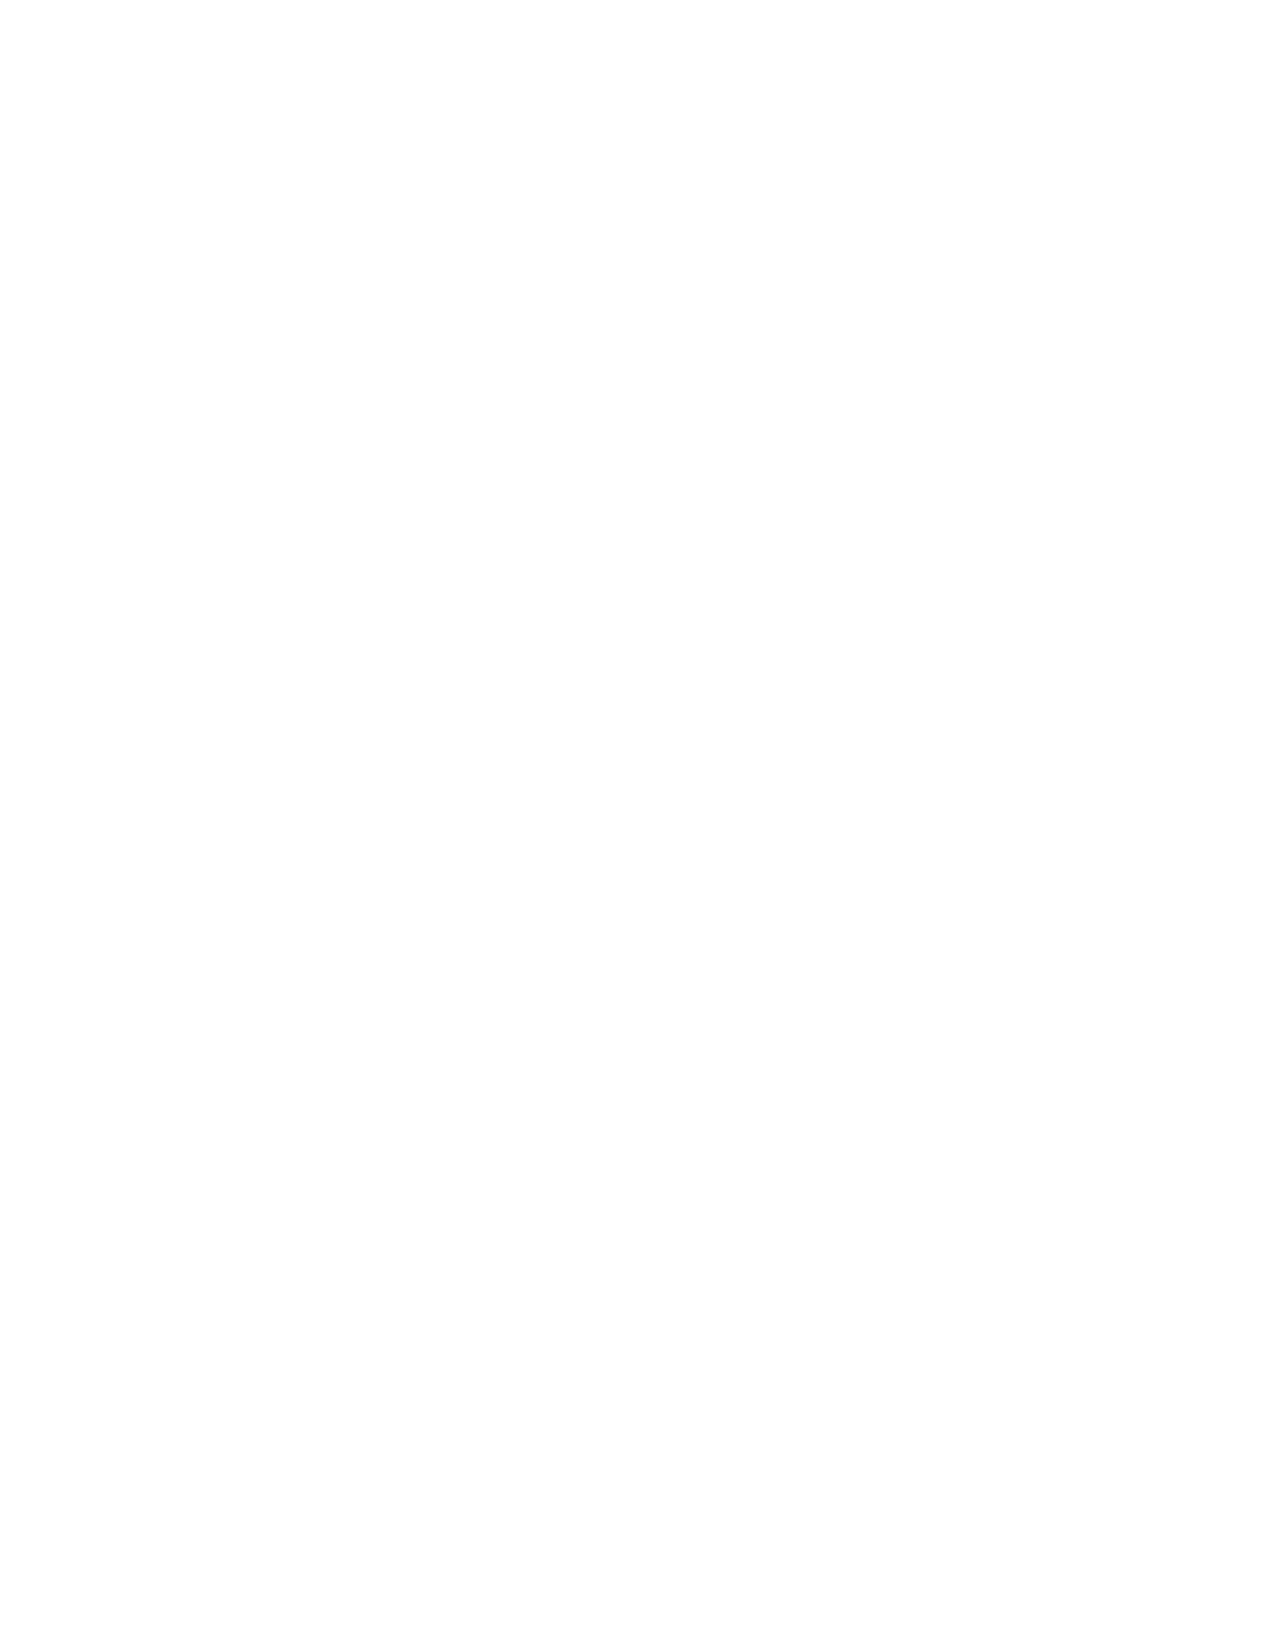
\includegraphics[max width=\textwidth]{2022_01_06_73aade67e8906ae5893fg-2}

\section{Convolutional Neural Networks}
\subsection{Some classic CNN models}
In this section, we will use these convolutional operations introduced above to give a brief description of some classic convolutional neural network (CNN) models. Firstly, CNNS are actually a class of special DNN models. Let us recall the DNN structure as:
$$
\begin{cases}f^{0}(x) & =x \\ f^{\ell}(x) & =\sigma\left(\theta^{\ell}\left(f^{\ell-1}\right)\right) \quad \ell=1: L \\ f(x) & =W^{L} f^{L}+b^{L}\end{cases}
$$
where
$$
\left(\theta^{\ell}\left(f^{\ell-1}\right)=W^{\ell} f^{\ell-1}(x)+b^{\ell} .\right.
$$
So the key features of CNNs is

    \begin{enumerate}
      \item Replace the general linear mapping to be convolution operations with multichannel.

      \item Use multi-resolution of images as shown in the next diagram.

    \end{enumerate}
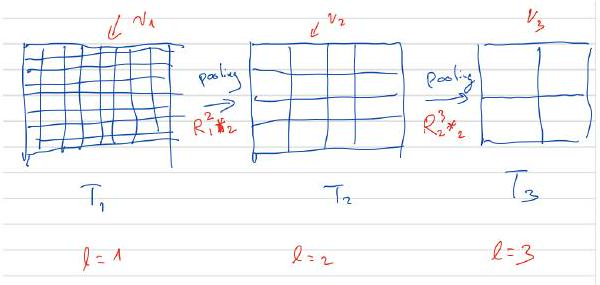
\includegraphics[max width=\textwidth]{2022_01_06_73aade67e8906ae5893fg-3}

Then we will introduce some classical architectures in convolution neural networks.

\subsubsection{LeNet-5, AlexNet and VGG}
The LeNet-5 $[6]$, AlexNet $[5]$ and VGG $[7]$ can be written as:

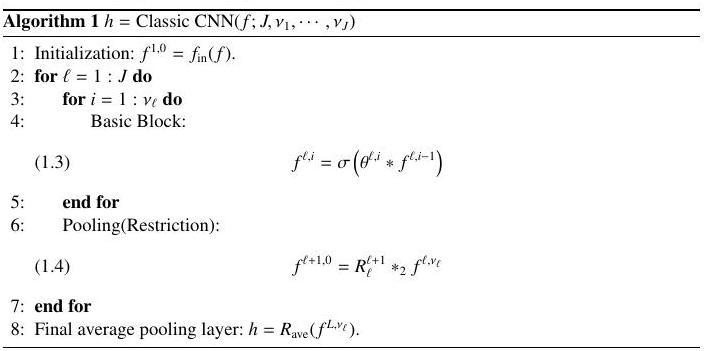
\includegraphics[max width=\textwidth]{2022_01_06_73aade67e8906ae5893fg-4}

Here $R_{\ell}^{\ell+1} *_{2}$ represents for the pooling operation to sub-sampling these tensors into coarse spatial level (lower resolution). Here we use $R_{\ell}^{\ell+1} *_{2}$ to stand for the pooling operation. In general we can also have

    \begin{itemize}
      \item average pooling: fixed kernels such as
    \end{itemize}
$$
R_{\ell}^{\ell+1}=\frac{1}{9}\left(\begin{array}{lll}
1 & 1 & 1 \\
1 & 1 & 1 \\
1 & 1 & 1
\end{array}\right)
$$

    \begin{itemize}
      \item Max pooling $R_{\max }$ as discussed before.
    \end{itemize}
In these three classic CNN models, they still need some extra fully connected layers after $h$ as the output of CNNs. After few layers of fully connected layers, the model is completed by following a multi-class logistic regression model.

These fully connected layers are removed in ResNet to be described below.

\subsubsection{ResNet}
The original ResNet developed in [2] is one of the most popular CNN architectures in image classification problems.

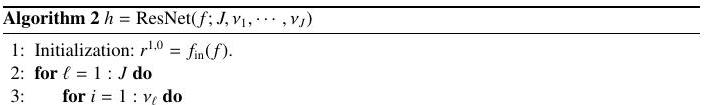
\includegraphics[max width=\textwidth]{2022_01_06_73aade67e8906ae5893fg-4(1)}

4: Basic Block:

(1.6) $r^{\ell, i}=\sigma\left(r^{\ell, i-1}+A^{\ell, i} * \sigma \circ B^{\ell, i} * r^{\ell, i-1}\right)$.

5: end for

6: Pooling(Restriction):

(1.7) $r^{\ell+1,0}=\sigma\left(R_{\ell}^{\ell+1} *_{2} r^{\ell, v_{\ell}}+A^{\ell+1,0} \circ \sigma \circ B^{\ell+1,0} *_{2} r^{\ell, v_{\ell}}\right) .$

7: end for

8: Final average pooling layer: $h=R_{\text {ave }}\left(r^{L, v_{t}}\right)$.

Here $f_{\text {in }}(\cdot)$ may depend on different data set and problems such as $f_{\text {in }}(f)=\sigma \circ \theta^{0} * f$ for CIFAR [4] and $f_{\text {in }}(f)=R_{\max } \circ \sigma \circ \theta^{0} * f$ for ImageNet [1] as in [3]. In addition $r^{\ell, i}=r^{\ell, i-1}+A^{\ell, i} * \sigma \circ B^{\ell, i} * \sigma\left(r^{i-1}\right)$ is often called the basic ResNet block. Here, $A^{\ell, i}$ with $i \geq 0$ and $B^{\ell, i}$ with $i \geq 1$ are general $3 \times 3$ convolutions with zero padding and stride 1. In pooling block, $*_{2}$ means convolution with stride 2 and $B^{\ell, 0}$ is taken as the $3 \times 3$ kernel with same output channel dimension of $R_{\ell}^{\ell+1}$ which is taken as $1 \times 1$ kernel and called as projection operator in [3]. During two consecutive pooling blocks, index $\ell$ means the fixed resolution or we $\ell$-th grid level as in multigrid methods. Finally, $R_{\mathrm{ave}}$ $\left(R_{\max }\right)$ means average (max) pooling with different strides which is also dependent on datasets and problems.

\subsection{3 pre-act ResNet}
The pre-act ResNet [3] shares a similar structure with ResNet.

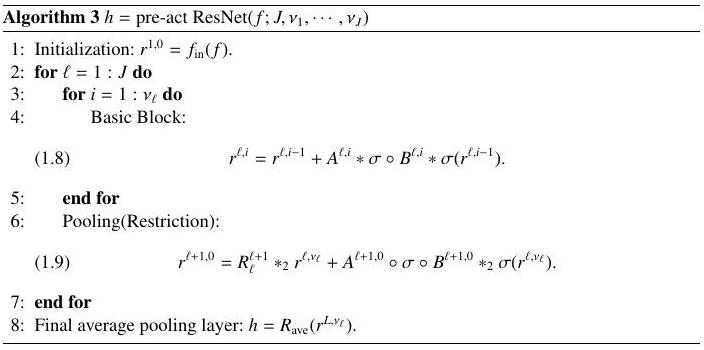
\includegraphics[max width=\textwidth]{2022_01_06_73aade67e8906ae5893fg-5}

Here pre-act ResNet share almost the same setup with ResNet.

The only difference between ResNet and pre-act ResNet can be viewed as putting a $\sigma$ in different places. The connection of those three models are often shown with next diagrams:

Without loss of generality, we extract the key feedforward steps on the same grid in different CNN models as follows.

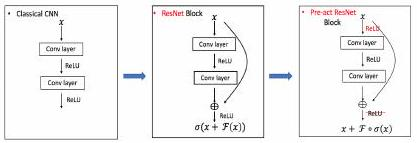
\includegraphics[max width=\textwidth]{2022_01_06_73aade67e8906ae5893fg-6}

Fig. 1.1. Comparison of CNN Structures

Classic CNN
$$
f^{\ell, i}=\xi^{i} \circ \sigma\left(f^{\ell, i-1}\right) \quad \text { or } \quad f^{\ell, i}=\sigma \circ \xi^{i}\left(f^{\ell, i-1}\right)
$$
ResNet
$$
r^{\ell, i}=\sigma\left(r^{\ell, i-1}+\xi^{\ell, i} \circ \sigma \circ \eta^{\ell, i}\left(r^{\ell, i-1}\right)\right)
$$
pre-act ResNet
$$
r^{\ell, i}=r^{\ell, i-1}+\xi^{\ell, i} \circ \sigma \circ \eta^{\ell, i} \circ \sigma\left(r^{\ell, i-1}\right)
$$

\section{References}
[1] J. Deng, W. Dong, R. Socher, L.-J. Li, K. Li, and L. Fei-Fei. Imagenet: A largescale hierarchical image database. In 2009 IEEE conference on computer vision and pattern recognition, pages 248-255. Ieee, 2009.

[2] K. He, X. Zhang, S. Ren, and J. Sun. Deep residual learning for image recognition. In Proceedings of the IEEE Conference on Computer Vision and Pattern Recognition, pages $770-778,2016$

[3] K. He, X. Zhang, S. Ren, and J. Sun. Identity mappings in deep residual networks. In European Conference on Computer Vision, pages 630-645. Springer, $2016 .$

[4] A. Krizhevsky and G. Hinton. Learning multiple layers of features from tiny images. Technical report, Citeseer, $2009 .$

[5] A. Krizhevsky, I. Sutskever, and G. E. Hinton. Imagenet classification with deep convolutional neural networks. In Advances in neural information processing systems, pages $1097-1105,2012$.

[6] Y. LeCun, L. Bottou, Y. Bengio, and P. Haffner. Gradient-based learning applied to document recognition. Proceedings of the IEEE, $86(11): 2278-2324,1998 .$

[7] K. Simonyan and A. Zisserman. Very deep convolutional networks for largescale image recognition. arXiv preprint arXiv: $1409.1556,2014 .$


\end{document}